\chapter{General Approach}
\label{sec:approach}


Given two surfaces $\mathcal{M}$ and $\mathcal{N}$, represented as triangulated meshes, the goal is to find the best match of  $\mathcal{N}$ (a partial shape) within  $\mathcal{M}$ (a full mesh).
In particular, we aim at extracting a sparse set of point correspondences between the shapes.
Our approach is based on the following four key ideas, of which the first two capture properties of the nearest-neighbor field in shape descriptor space between the surfaces.

%%%%%%%%%%%%%%%%%%%%Key Idea underlying the original DDIS : diversity
First, inspired by~\cite{talmi2017template}, 
when $\mathcal{N}$ and a part of $\mathcal{M}$ correspond, most points in that part of $\mathcal{M}$ have unique NN-matches in $\mathcal{N}$.
This implies that the NN field should be highly diverse, in the sense that many different points in $\mathcal{N}$ are being matched.
This is illustrated in Figure~\ref{fig:NNF}(a) where the two surfaces are equal and in Figure~\ref{fig:NNF}(b) where the two surfaces correspond, since one is a deformation of the other.
Therefore, in both of these cases, most points have unique matches and hence,  each line connects a different pair of points.
Conversely, Figure~\ref{fig:NNF}(d) shows a case of inherently-different surfaces, resulting in  a small number of target points that happen to be somewhat similar to the input points.


Second, arbitrary matches typically imply a large inconsistency in the location of the matches, whereas correct matches are consistent.
We propose to measure the degree of consistency by looking at the geodesic distances of points within a surface.
Specifically, when two surfaces correspond, the pairwise geodesic  distances between a reference point and other vertices in that surface should match the pairwise distances between the reference point and other vertices on the other surface.
In Figure~\ref{fig:NNF} this is encoded by the color of the lines that connect the two shapes.
In Figure~\ref{fig:NNF}(a,b), which show corresponding surfaces, the pairwise distances from their reference points are similar, and hence  they are colored in blue.
Conversely, in Figure~\ref{fig:NNF}(c,d), the colors of the lines indicate inconsistent  distances between the corresponding points, and many of the lines are yellow or cyan, as expected since the surfaces are non-corresponding.
Combining the above two ideas leads to a new similarity measure, which is based both on the diversity of the Nearest-Neighbor field and on the consistency of the distances between the points.
\begin{figure}[h!]
	\centering
	\setlength\tabcolsep{2pt}
	\begin{tabular}{ccc}
		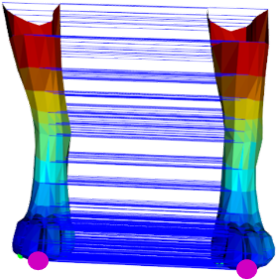
\includegraphics[width=0.2\textwidth]{figures/DDISsame.png} &
		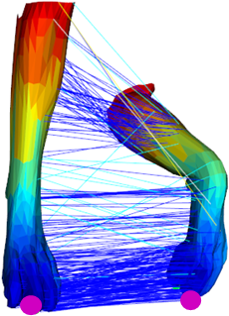
\includegraphics[width=0.16\textwidth]{figures/DDISdeformed.png}&
		\multirow{3}{*}[2.2cm]{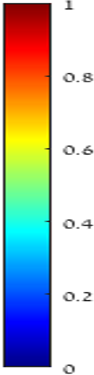
\includegraphics[height=0.25\textheight]{figures/colorbarDDIS.png}}\\
		(a) Same surface& (b) Deformed surface &\\
		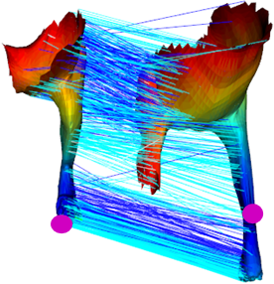
\includegraphics[width=0.2\textwidth]{figures/DDIS_shifted.png} &
		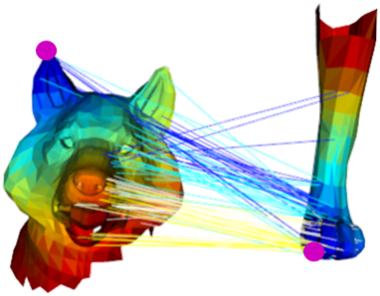
\includegraphics[width=0.22\textwidth]{figures/DDISunrelated.png}&\\
		(c) Shifted surface & (d) Different surfaces & $\sqrt{Area(\mathcal{M})}$
	\end{tabular}
	
	\caption{{\textbf{Properties of the nearest-neighbor field.}}
	The surfaces are colored by their geodesic distances from the magenta reference point (center of the surface); the lines are colored by the difference between the geodesic distances from the reference point of the corresponding pairs of points.
	Clearly, similar surfaces (a,b), even when deformed, exhibit diversity in matching.
	This can be seen by the fact that the points of the corresponding pairs, connected by lines, are all distinct, rather than having some point(s) into which many lines converge.
	Furthermore, in this case, most lines are blue, which indicates similar distances from the reference point.
	Conversely, in (c), though the surfaces are similar, the reference point is different.
	In this case there are many cyan lines, indicating a worse correspondence due to  bad localization.
	Finally, when the surfaces are highly different (d), there are many yellow and cyan lines, indicating bad correspondence.
}

	\label{fig:NNF}
\end{figure}

Third, rather than realizing the above two ideas on $\mathcal{N}$ as a whole, it is preferable to perform it on a set of smaller sub-surfaces of $\mathcal{N}$.
This is due to two reasons:
(1)~A small sub-surface is more likely to exhibit consistent distances, especially in the presence of partiality, holes or topological noise.
For instance, take two corresponding vertices, one on a full surface and the other on a surface with holes; the geodesic distances between each of these vertices and other vertices on their associated surfaces will greatly vary, as a result of "bypassing" holes.
(2)~In the case of repeating patterns and a large surface, the diversity will be small, contrary to what we seek-after. 

Fourth, a multi-scale approach with respect to the size of matched sub-surfaces is beneficial ~\cite{raviv2011hierarchical}.
This is so since larger surfaces contain more global context, resulting in matches which lie within the correct region, but provide poor localization.
On the other hand, matching smaller surfaces leads to results that are better locally, but may be globally inconsistent (e.g., mapping a hind leg to a front leg, which is identical locally).



\begin{figure*}[htb]
	\centering
	\setlength\tabcolsep{2pt}
	\begin{tabular}{ccccccc}
		$\mathcal{M}$&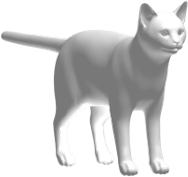
\includegraphics[width=0.125\textwidth]{figures/BirdsFlightFull.png} &
		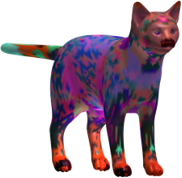
\includegraphics[width=0.125\textwidth]{figures/NNFout.png} &
		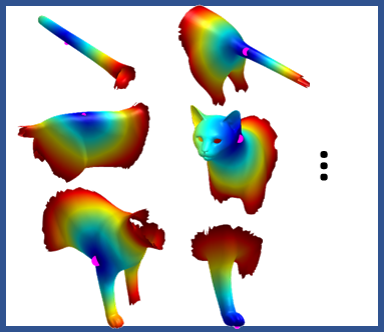
\includegraphics[width=0.2\textwidth]{figures/FullPatches.png} &
		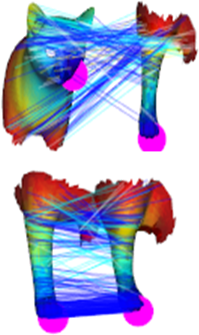
\includegraphics[width=0.1\textwidth]{figures/DDISup.png} &
		
\includegraphics[width=0.1\textwidth]{figures/CorrsBaseInit.png} &
		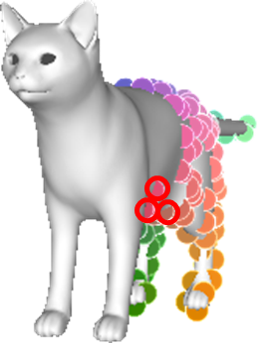
\includegraphics[width=0.1\textwidth]{figures/CorrsBaseOutlier.png}
		
\includegraphics[width=0.1\textwidth]{figures/CorrsBaseRefine.png}\\
		$\mathcal{N}$ &
\includegraphics[width=0.08\textwidth]{figures/BirdsFlightPart.png} &
		
\includegraphics[width=0.08\textwidth]{figures/NNFin.png} &
		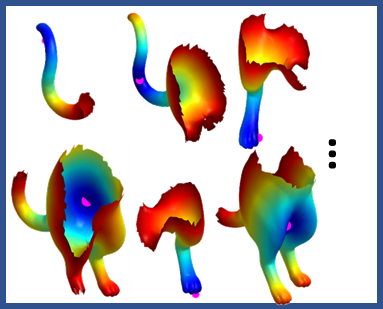
\includegraphics[width=0.2\textwidth]{figures/PartPatches.png} &
		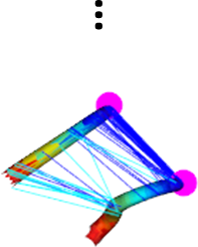
\includegraphics[width=0.1\textwidth]{figures/DDISdown.png} &
		
\includegraphics[width=0.1\textwidth]{figures/CorrsInit.png} &
		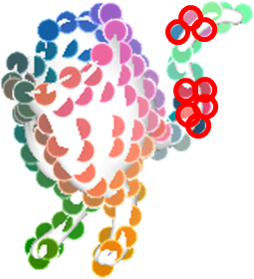
\includegraphics[width=0.1\textwidth]{figures/CorrsOutlier.png}
		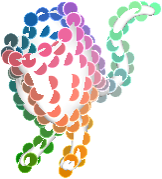
\includegraphics[width=0.1\textwidth]{figures/CorrsRefine.png}\\
		&input &
		Step 1: &
		Step 2:  &
		Step 3:  &
		Step 4:  &
		Step 5: 
		\\
		& &
		 NN &
		 patch extraction &
		 similarity &
		 correspondence &
		 refinement
	\end{tabular}
	\caption{{\textbf {Algorithm outline.}}
    In Step~1, we compute the nearest-neighbor field that maps the shape descriptors of $\mathcal{M}$ to their corresponding nearest neighbors on~$\mathcal{N}$.
In Step~2, sub-surfaces (patches) are extracted for every sample point in $\mathcal{N}$ and for every vertex in $\mathcal{M}$.
Examples of six such patches are shown; note that they may overlap.
A reference point on each subsurface is shown in magenta and the colors on the surface encode the geodesic distance from it.
Step~3, which is the core of the algorithm, computes the similarity between the patches in $\mathcal{M}$ and $\mathcal{N}$.
In the figure, the nearest neighbors are connected by lines.
The color of the lines encodes the difference of the geodesic distances between each of these vertices and the reference point in its own subsurface.
In Step~4, the color of the points represent their correspondence--- points that achieve the maximal similarity score are corresponding (and have the same color on both models).
Step~5 refines the correspondences, by modifying the outliers according to the correspondences in their environment.
See, for instance, the changes of the corresponding points of those marked by red circles.
	}
	\label{fig:overview}
\end{figure*}

Our algorithm, which is illustrated in Figure~\ref{fig:overview}, realizes these ideas. It consists of five steps, as follows.

%%%%%%%%%%%%% Step 1
\vspace{0.1in}
\noindent
\textbf{1. Descriptors \& Nearest-Neighbors.}
Shape descriptors are calculated for every vertex of both meshes.
Many descriptors have been proposed in the literature~\cite{rusu2008towards,tombari2010unique,Sun:2009:CPI:1735603.1735621}.
We use the {\em Fast Point Feature Histogram (FPFH)}~\cite{rusu2009fast}, which captures the relative angular directions of the normals with respect to one another.
FPFH is robust to small deformations and partiality of the data, whilst sensitive to symmetrical flips, since it relies on the angles between many local reference frames around each point~\cite{shtrom2013saliency}.
Therefore, it addresses a major drawback of matching a right arm, for example, to the left one.

%
We then compute an approximate nearest neighbor field (\textit{NNF}) mapping.
This is done by assigning each vertex of $\mathcal{M}$ its nearest neighbor in $\mathcal{N}$, in terms of their FPFH descriptors.

%%%%%%%%%%%%% Step 2
\vspace{0.1in}
\noindent
{\textbf {2. Patch extraction.}}
Inline with the third key idea, we aim at extracting a meaningful set of sub-surfaces, which cover (rather than partition) the surface.
This is done in two steps:
First, we extract a meaningful set of sample points.
We then extract the patches using these samples.
We elaborate hereafter.

To extract the sample point set $S$, we start from the extremities of the surface, which are considered salient points~\cite{katz2005mesh}.
A vertex is defined as an extremity if it  resides on a tip of the surface (e.g.,  tips of limbs),
In practice, we define an extremity to be a vertex that is a local maximum of the sum of the geodesic distance functional.

Formally, $\forall v \in \mathcal{N}$,  let $N_v$ be the set of neighboring vertices of vertex $v$.
Let $GeoDist(v_i, v_j)$ be the geodesic distance between vertices $v_i$ and $v_j$ on mesh $\mathcal{N}$. 
Vertex $v$ is an extremity if it satisfies
\begin{equation}
	\sum_{v_i\in \mathcal{N}} GeoDist(v,v_i)>\sum_{v_i\in \mathcal{N}} GeoDist(v_n, v_i)~\forall v_n\in N_v.
	\label{eq:extremities}
\end{equation}

Then, we iteratively add more samples,so as to gradually cover more and more of the mesh.
At each iteration, the next sample point is chosen as follows.
We construct a "forbidden" region around every point in the set.
This region is a geodesic disc of radius $ 0.05\sqrt{Area(\mathcal{M})}$; the constant is chosen so as the number of points would be on par with other sparse methods~\cite{cosmo2016shrec}.
The next point to be added to the set is a vertex whose geodesic distance to any sample point is minimal and it must not fall in any of the forbidden regions.
This process stops when the entire surface is marked forbidden.

Once the set of representing samples is defined, a disc (sub-surface) of geodesic radius $R_T$ is extracted around each sample point.
This is the sought-after set of patches that covers the surface.
Specifically,~$R_T=\beta\cdot \sqrt{Area(\mathcal{M})}$.
As our approach is multi-scale,~$\beta$, which was found empirically by minimizing the error of correspondences on a training set, varies.
In practice we use~$\beta=\{0.6,0.4,0.2\}$.




%%%%%%%%%%%%% Step 3
\vspace{0.1in}
\noindent
{\textbf {3. Computing similarities between pairs of patches.}}
This step is the core of our algorithm, which realizes the first two key ideas.

For each pair of patches of the same scale, $P_i \subset \mathcal{N}$ and $Q_j \subset \mathcal{M}$, constructed around vertices $v_i$ and $w_j$ respectively, as described in Step 2, we compute a similarity value.
%
Recall that our goal is to reward a nearest-neighbor field with high diversity and low inconsistency.
We will define the similarity function that achieves it  in Section~\ref{sec:similarity}.
We note that this step, as well, is performed in a multi-scale manner.


%%%%%%%%%%%%% Step 4
\vspace{0.1in}
\noindent
{\textbf {4. Extracting a sparse set of corresponding points.}}
Given the similarity values between the patches, as computed in Step~3, our goal now is to extract a set of corresponding points between  $\mathcal{N}$ and $\mathcal{M}$.
If we had a single scale, then for each sample point (the center of a patch) of~$\mathcal{N}$, we would choose the vertex of $\mathcal{M}$ that maximizes the similarity function.
However, if the scale is too coarse, the exact matching point is likely not to be found; and if the scale is too fine we may find a corresponding vertex, but on other parts of the model (e.g., on almost-symmetric parts).

Our multi-scale approach addresses these difficulties.
We proceed from coarse to fine, first finding the most likely region the corresponding point should lie on and then refining the exact location.
Suppose that $P_i \subset \mathcal{N}$ and $Q_j\subset \mathcal{M}$ were found to have the highest similarity in a coarsest scale.
The coarsest correspondence is then set between $v_i \in P_i$ and $w_j \in Q_j$, where $v_i, w_j$ are the {\em geodesic centers} of  $P_i, Q_j$, respectively (i.e. these are the sample points that define the patches in Step 2).
When moving to a finer scale, we replace  $Q_j$ with a smaller patch in which $w_j$ is the center.
Once this patch is constructed, we replace the vertex $w_j$ by a new vertex $w_{j_n}$.
The latter is set to be the vertex on the patch that maximizes the similarity function of Stage~3 for this patch.
Since $w_{j_n}$ is more similar to $v_i$ than any other vertex on the patch, it is considered to be the new corresponding point of $v_i$.
Recall that vertex $w_{j_n}$ corresponds to $v_i$ on a patch smaller than the one associated with $w_j$.
In this manner we move from one scale to the next and refine the corresponding vertex of $v_i$.

Figure~\ref{fig:multiscale} illustrates how the correspondence found at the first scale  improves throughout the scales.
This is compared to the case in which a single scale is used and the corresponding point is either inexact ($\beta=0.6$) or is erroneous ($\beta=0.4,0.2$) .
\begin{figure}[htb]
	\centering
	\begin{tabular}{c|ccc|c}
		
		\multirow{ 3}{*}{ { 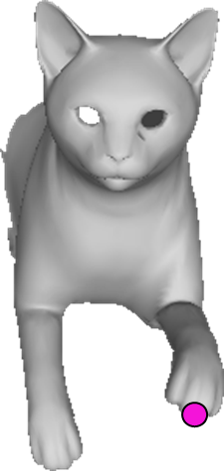
\includegraphics[width=0.06\textwidth]{figures/Original.png}}}
		&
		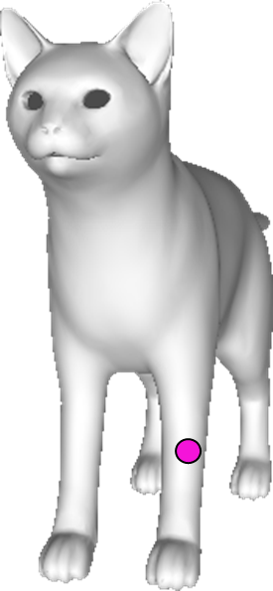
\includegraphics[width=0.07\textwidth]{figures/B0_6result.png} &
		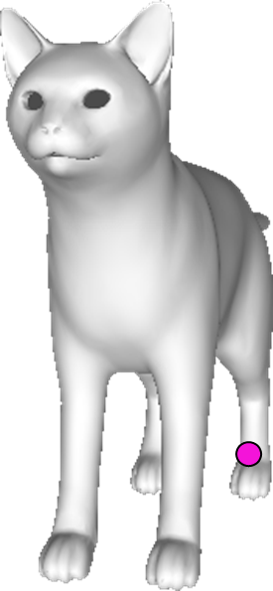
\includegraphics[width=0.07\textwidth]{figures/B0_4result.png} &
		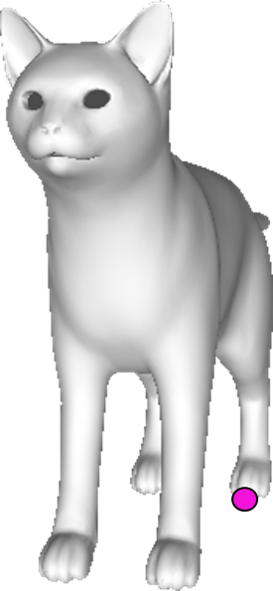
\includegraphics[width=0.07\textwidth]{figures/B0_2result.png} & \rotatebox{90}{Single scale results}
		\\
		& $\beta=0.6$ & $\beta=0.4$ & $\beta=0.2$ \\
		\cline{2-5}
		&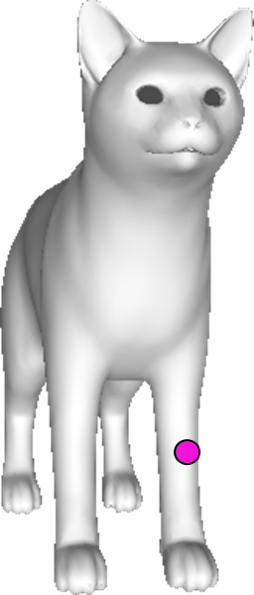
\includegraphics[width=0.07\textwidth]{figures/B0_6MSDIS.png} &
		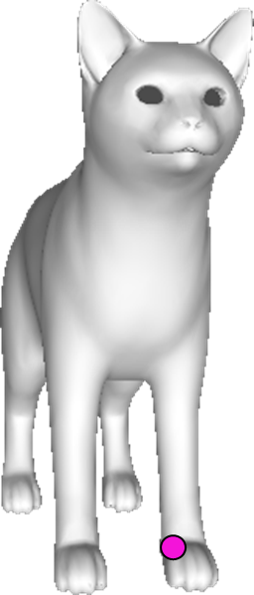
\includegraphics[width=0.07\textwidth]{figures/B0_4MSDIS.png} &
		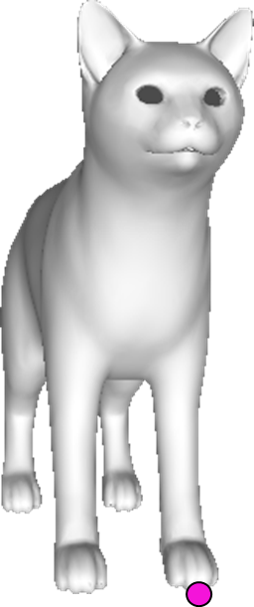
\includegraphics[width=0.07\textwidth]{figures/B0_2MSDIS.png} &
		\rotatebox{90}{Multi scale results} \\
		& $\beta=0.6$ & $\beta=0.4$ & $\beta=0.2$ \\ \hline
		$\mathcal{N}$ & \multicolumn{3}{c}{$\mathcal{M}$}
	\end{tabular}
	\caption{{\textbf{ Multi-scale similarity.}}
	The input is the the sample point on the left (in magenta).
In the coarsest level ($\beta=0.6)$), the region of the corresponding point is found, but the point itself is imprecise.
In a single-scale approach (top row), finer scales miss the correct region altogether.
Conversely, our multi-scale approach (bottom row) utilizes the coarse corresponding region to keep refining the correspondence, and the precise correspondence is found in the finest scale.
	}
	\label{fig:multiscale}
	
\end{figure}

%%%%%%%%%%%%%%% Step 5
\vspace{0.1in}
\noindent
{\textbf{ 5. Coherency-based correspondence refinement.}}
The result of Step~4 is a set of corresponding pairs of points.
In most cases ($>92\%$ in all our examples), the correspondences are correct.
The goal of this step is to identify the incorrect ones and replace them by the correct correspondences.

The key idea is to utilize coherency, i.e., if all points in the neighborhood of point $v \in \mathcal{N}$ are mapped to points that reside in the same region on $\mathcal{M}$,  it is expected that the corresponding point of $v$,  $w \in \mathcal{M}$, will also reside in this region.
In other words, we are looking for outliers of the mapping in order to fix them.

To detect these outliers, we check the sum of difference of geodesic distances induced by the mapping  between a pair of points in $\mathcal{N}$ and their corresponding points in $\mathcal{M}$. 
On average, outliers will result in a large difference of geodesic distances and can therefore be detected by an empirically-set threshold.
Let us define the sum of differences of geodesic distances between a point $v_j \in \mathcal{N}$ and its corresponding point $w_j \in \mathcal{M}$ as
\begin{equation}
	\centering
	\label{eq:refinement}
	\Delta_{v_j,w_j}=\sum_{v_i\in S}|{GeoDist(v_j,v_i)} - {GeoDist(w_j,w_i)}|,
\end{equation}
where $w_i$ is the corresponding point of $v_i$.
We consider a correspondence $(v_j,w_j)$ to be correct if it is smaller than the average distance of all other correspondences,
\begin{equation}
	\centering
	\label{eq:refinement2}
	\Delta_{v_j,w_j}<C\frac{\sum_{v_i\in S}\Delta_{v_i,w_i}}{|S|},
\end{equation}
where $C$ is empirically set to $1.15$.

If Equation~\ref{eq:refinement2} is violated, it indicates geodesic distance inconsistency with many other correspondences, thus, $v_j$ is considered an outlier.
In this case, we replace $w_j$, the corresponding point of $v_j$, by a "better" point $w_j*$.
We require this point to satisfy two conditions:
(1) it is a local maximum of the similarity function of Step~3 (to be discussed hereafter in Section~\ref{sec:similarity}) and (2) among the vertices that satisfy condition~(1) we choose as $w_j*$ the vertex whose $\Delta_{v_j,w_j*}$ is minimal.
The first condition means that the two vertices are indeed similar.
The second condition means that the correspondence is consistent.
